	\newpage
\section{Wnioski}	%5
%Npisać wnioski końcowe z przeprowadzonego projektu, 

\subsection{AI}
Nie należy ignorować narzędzi AI jak Copilot i uznawać je jako jakieś tymczasowe zabawki dla deweloperów, które kiedyś wyjdą z mody. Nawet w swoim obecnym stanie, sam fakt, że po napisaniu \texttt{for}, jednym kliknięciem taba, \textit{najprawdopodobniej} Copilot wytworzy nam sensowną pętle \textit{biorąc pod uwagę kontekst szerszego programu} jest bez dwóch zdań bardzo użyteczny, po prostu przez to, że oszczędza to programiście czas. Ponadto, narzędzia te są świetnymi wyszukiwarkami, co szczególnie się tyczy modeli, które mają dostęp do internetu. Nie trzeba praktycznie walczyć z zareklamowanym po kark Google i przeszukiwać napisanych przez boty stron - taki model automatycznie "przesieje" internet i pokaże nam informacje, które faktycznie dotyczą naszego zapytania. No, chyba że o to co się pytamy jest rzeczą niszową.

Niektórym (najbardziej to inwestorom w firmy zajmujące się AI) wydaje się, że LLM może za człowieka myśleć. Po części to prawda - jeżeli przed modelem o danym problemie myśleli inni - im więcej głowili się tym lepiej - i te przemyślenia gdzieś upublicznili, to LLM błyskawicznie może sięgnąć po tego problemu rozwiązanie. Ba, może nawet je po części zmodyfikować. Problem pojawia się, jeżeli zaczniemy naciskać na biednego chatbota. Fakty są następujące: LLM potrzebuje bardzo dużej ilości informacji o danym koncepcie, aby go opanować oraz LLM słabo potrafi rozumować, to jest, syntezować znane już informacje w nowe. Praktycznie, objawia się to gdy zapytamy się czatbota o rzecz, o której się mało mówi. 

Osobiście mogę przytoczyć przykład próby zrozumienia API \texttt{pipewire}\cite{pipewiresite}. Jest to projekt zajmujący się zarządzaniem strumieniami audio (takimi z aplikacji) na Linuxie. Rzecz, z natury niszowa. Chciałem przechwycić wyjście jednej aplikacji i uzyskać na bieżąco sample jakie wysyła. Ile to było bawienia się z ChatemGPT, prób wyplucia przez niego programu który się nie segfaultuje - głównie dlatego, że nie chciało mi się czytać dokumentacji. Czat podczas treningu pewnie przeczytał - ale mało co z tego wyciągnął, bo strona z API to było jedno z niewielu miejsc, gdzie owo API było opisane. W końcu okazało się, że na stronie był przykład programu, który robił prawie to samo co chciałem i jedyne co ChatGPT mi dał to powód do przeczytania dokumentacji. 

Pytać się można czy LLMy zastąpią programistów. Wydaje mi się, że - jeżeli nie teraz to za parę lat - programiści, których praca składa się z kopiowania zapytań o najnowszy framework JS ze Sack Overflowa i wklejania, faktycznie są zagrożeni, bo LLMy właściwie robią to, ale szybciej i taniej. Lecz programiści, którzy faktycznie tworzą coś nowego, faktycznie tworzą projekty wcześniej niedokonane, stoją na czele innowacji lub nią są - nie mają się czym martwić na długo.

Dotknąłem już do czego funkcja czatu może być użyteczna. W tym akurat zadaniu użyłem ChataGPT do pokazania faktycznej matematyki za algorytmem. Widać jego wypowiedź na rysunku nr.~\ref{fig:chatgptpcalka} 

\begin{figure}[H]
	\centering
	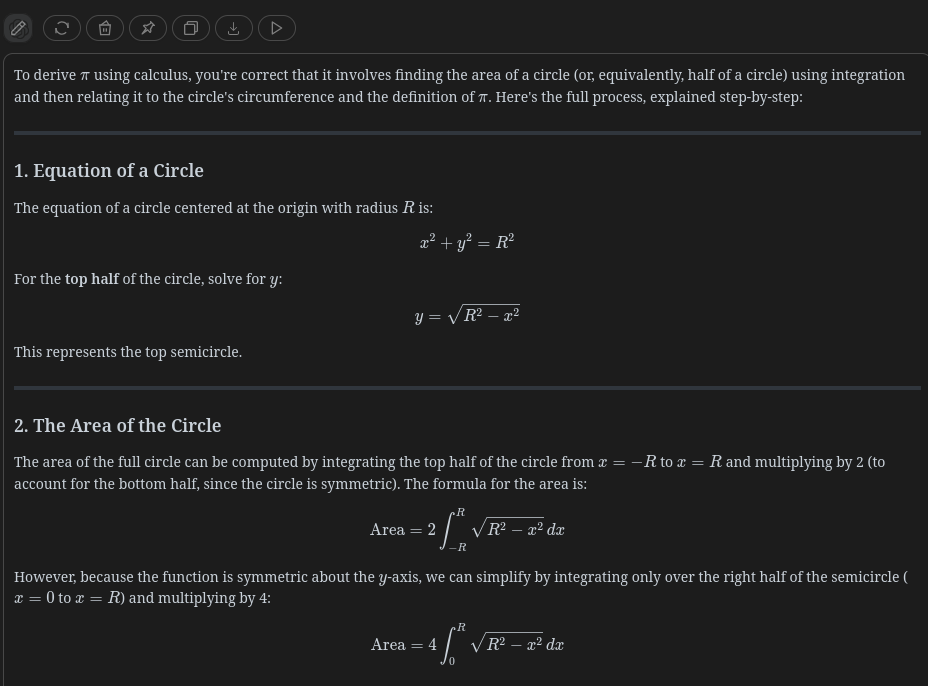
\includegraphics[width=1\textwidth]{images/chatgpt_calka.png}
	\caption{\centering{Wypowiedź Chata na temat sposobu obliczania pola pod kołem.}}
	\label{fig:chatgptpcalka}
\end{figure}

Wypowiedź z rysunku nr.~\ref{fig:chatgptpcalka} została wygenerowana modelem \texttt{gpt4o}.

\subsection{Wykonanie programu}

Program wykonuje się jak należy i kalkuluje $\pi$. Lecz warto zauważyć, że dla większej liczby wątków precyzja spada. Można to zauważyć na listingu nr. \ref{lst:accuracy}

\begin{lstlisting}[caption=Funkcja \texttt{getPi()}, label={lst:accuracy}, language=plaintext]
Select the accuracy of the algorithm (rectangles in a quarter of the circle): 10000000

Select the number of threads to use: 1

Calculated Pi: 3.141592853552536

------

Select the accuracy of the algorithm (rectangles in a quarter of the circle): 10000000

Select the number of threads to use: 50

Calculated Pi: 3.1415936525118267
\end{lstlisting}

Wartość $\pi$ to ok. $3.141592653589793$. Porównując 13 i ostatnią linijkę, dla 50 wątków, wartość $\pi$ jest mniej dokładna niż dla 1 wątku. Może to wynikać z tego, że wątki nie są synchronizowane, a więc mogą się zdarzyć przypadkowe kolizje, które zniekształcają wynik.

\subsection{Benchmarki}

Szersza implementacja benchmarków została opisana w sekcji nr.~\ref{sec:benchmarkimpl}. Benchmarki zostały przeprowadzone w dwóch zbiorach. Pierwszy, z wykresem na rysunku nr.~\ref{fig:benchmarklowc} pokrył zakres od 1 do \texttt{5'000'000'000} iteracji i 1 do 12 wątków (tyle jest na maszynie testującej). Drugi wykres którego jest zawarty na rysunku nr.~\ref{fig:benchmarkhighc}, testował od 1 do 50 wątków, ale ograniczony był do \texttt{1'000'000'000} iteracji, w celu oszczędzenia czasu. Osi \texttt{y} wykresów to suma wszystkich iteracji funkcji benchmarkującej dla danej ilości wątków. Oś \texttt{x} to po prostu ilość wątków użyta w benchmarku.

\begin{figure}[H]
	\centering
	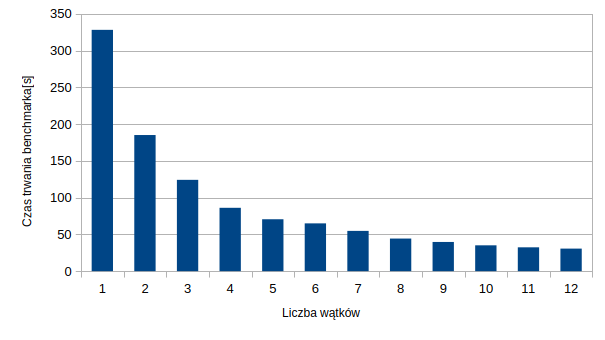
\includegraphics[width=1\textwidth]{images/benchmarks_lowc.png}
	\caption{\centering{Benchmark z niepełnym zakresem wątków}}
	\label{fig:benchmarklowc}
\end{figure}

\begin{figure}[H]
	\centering
	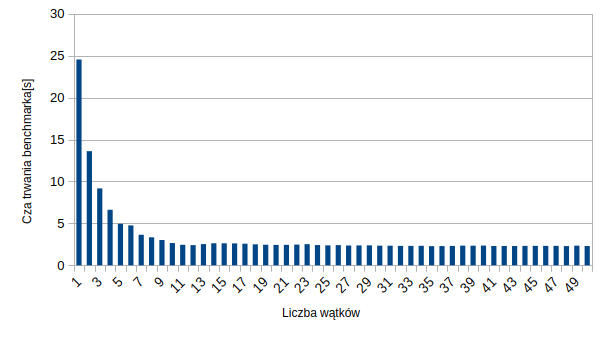
\includegraphics[width=1\textwidth]{images/benchmarks_highc.png}
	\caption{\centering{Benchmark z pełnym zakresem wątków}}
	\label{fig:benchmarkhighc}
\end{figure}

Jak widać na rysunku nr.~\ref{fig:benchmarklowc} wraz ze zwiększeniem liczby wątków, czas benchmarku zmniejsza się wykładniczo. Na rysunku nr. \ref{fig:benchmarkhighc} dzieje się podobnie, dopóki benchmark nie dojdzie do większej ilości wątków niż 12. Wtedy, czas wykonywania lekko wzrasta. Może się to dziać ponieważ tworzone jest więcej obiektów wątku, ale nie są one wykorzystywane przez procesor, co sprawia, że niepotrzebnie nakładany jest dodatkowy overhead.
